\documentclass[conference]{IEEEtran}
\IEEEoverridecommandlockouts
% The preceding line is only needed to identify funding in the first footnote. If that is unneeded, please comment it out.
\usepackage{cite}
\usepackage{amsmath,amssymb,amsfonts}
\usepackage{algorithmic}
\usepackage{graphicx}
\usepackage{textcomp}
\usepackage{xcolor}
\usepackage{multirow}
\usepackage{float}
\usepackage[english]{babel} % To obtain English text with the blindtext package
\usepackage{blindtext}
\def\BibTeX{{\rm B\kern-.05em{\sc i\kern-.025em b}\kern-.08em
    T\kern-.1667em\lower.7ex\hbox{E}\kern-.125emX}}
\begin{document}

\title{Understanding the effect of Hyperparameter optimisation in Neural Networks}

\author{\IEEEauthorblockN{Sivaram Ainkaran}
\IEEEauthorblockA{\textit{School of Mathematics \& Statistics} \\
\textit{University of New South Wales}\\
Sydney, Australia \\
s.ainkaran@student.unsw.edu.au}
}

\maketitle

\begin{abstract}
Hyperparameter tuning is a required exercise in neural network training. It creates a model that is optimised for both performance and efficiency. It is, however, a costly exercise due to the number of hyperparameters which need to be adjusted and the time and computing power required for it.\textsuperscript{[2, p.2]}

This report, aims to evaluate the effect of different hyperparameter values on model performance and whether these variations provide statistically significant performance gain. The key hyperparameters tested were the number of neurons in hidden layers, the learning rate of a chosen optimiser, the number of hidden layers and the chosen optimiser itself.

The results provide insight into the effect of hyperparameter tuning and why it is such an important step in neural network training.
\end{abstract}

\begin{IEEEkeywords}
machine learning, neural network
\end{IEEEkeywords}

\section{Introduction}
If we go deep enough, there are an endless number of hyperparameters to be tuned, and each of these can affect the performance of a model. This report aims to explore these effects and whether they provide tangible differences in model performance. As models get larger, these optimisations become more and more important. For our tests, however, we will be using a simple 1 to 2 layer feed-forward neural network with up to 20 neurons per layer. Tests will also be conducted on different optimisers and various learning rates of this optimiser. 

Each hyperparameter selected for testing plays a crucial role in model optimisation. 

The number of neurons per hidden layer can greatly slow down model training but can provide a better performing model in the end. However, adding too many neurons increases the number of model parameters and can cause overfitting due to the bias-variance tradeoff, and the model can lose its generalising capabilities\textsuperscript{[8, p. 81]}. The same can be said for the number of hidden layers used.

The chosen learning rate of our optimiser greatly affects training time and model performance in different ways. If it is too small, training time increases and the model can get stuck in shallow minima, creating poor model accuracy. If it is too large, training will become unstable and the model may not converge. An optimal learning rate will be big enough to skip over shallow minima but small enough to get stuck in deeper, better minima.

Similar to learning rate, we must choose the optimiser that is the best for the job. Between our 2 optimisers, Adam is a much faster algorithm than Stochastic Gradient Descent, but it tends to perform worse in deep learning contexts, plateauing much earlier\textsuperscript{[9, p. 1]}. This may not be a factor in our simple neural networks, however.

The remaining sections will detail the methodology and discuss our findings.

\section{Methodology}
\subsection{Data set}
We trained the neural network on the \textit{Abalone} data set provided by the UC Irvine Machine Learning Repository\textsuperscript{[1]}. This data set contains information on 8 feature variables and 1 target variable of 4177 abalone. 

Features variables are:
\begin{description}
    \item \textbf{Sex} \textit{(categorical)}: Male, Female or Infant
    \item \textbf{Length} \textit{(continuous)}: Longest shell measurement
    \item \textbf{Diameter} \textit{(continuous)}: Shell measurement perpendicular to length
    \item \textbf{Height} \textit{(continuous)}: Shell height with meat inside
    \item \textbf{Whole weight} \textit{(continuous)}: Weight of whole abalone
    \item \textbf{Shucked weight} \textit{(continuous)}: Weight of meat
    \item \textbf{Viscera weight} \textit{(continuous)}: Weight of gut (after bleeding) 
    \item \textbf{Shell weight} \textit{(continuous)}: Weight of shell (after drying)
\end{description}


Target variable is:
\begin{description}
    \item \textbf{Rings} \textit{(integer)}: Number of rings in abalone shell
\end{description}
The target variable \textit{Rings} is found by ``cutting the shell [of an abalone] through the cone, staining it, and counting the number of rings through a microscope"\textsuperscript{[1]}. Adding 1.5 to the number of rings gives us the age of the abalone.

\subsection{Exploratory data analysis \& Preprocessing}
The data was processed to prepare a clear classification problem for our neural network to train on.

We reclassified \textit{Rings} into the following 4 classes:
\begin{itemize}
    \item Class \textbf{0}: Rings $\leq7$
    \item Class \textbf{1}: $7 < \text{Rings} \leq 10$
    \item Class \textbf{2}: $10 < \text{Rings} \leq 15$
    \item Class \textbf{3}: $15 < \text{Rings}$
\end{itemize}

The distribution of classes we created are shown in Figure~\ref{fig:classdist}.
\begin{figure}[htbp]
\centering
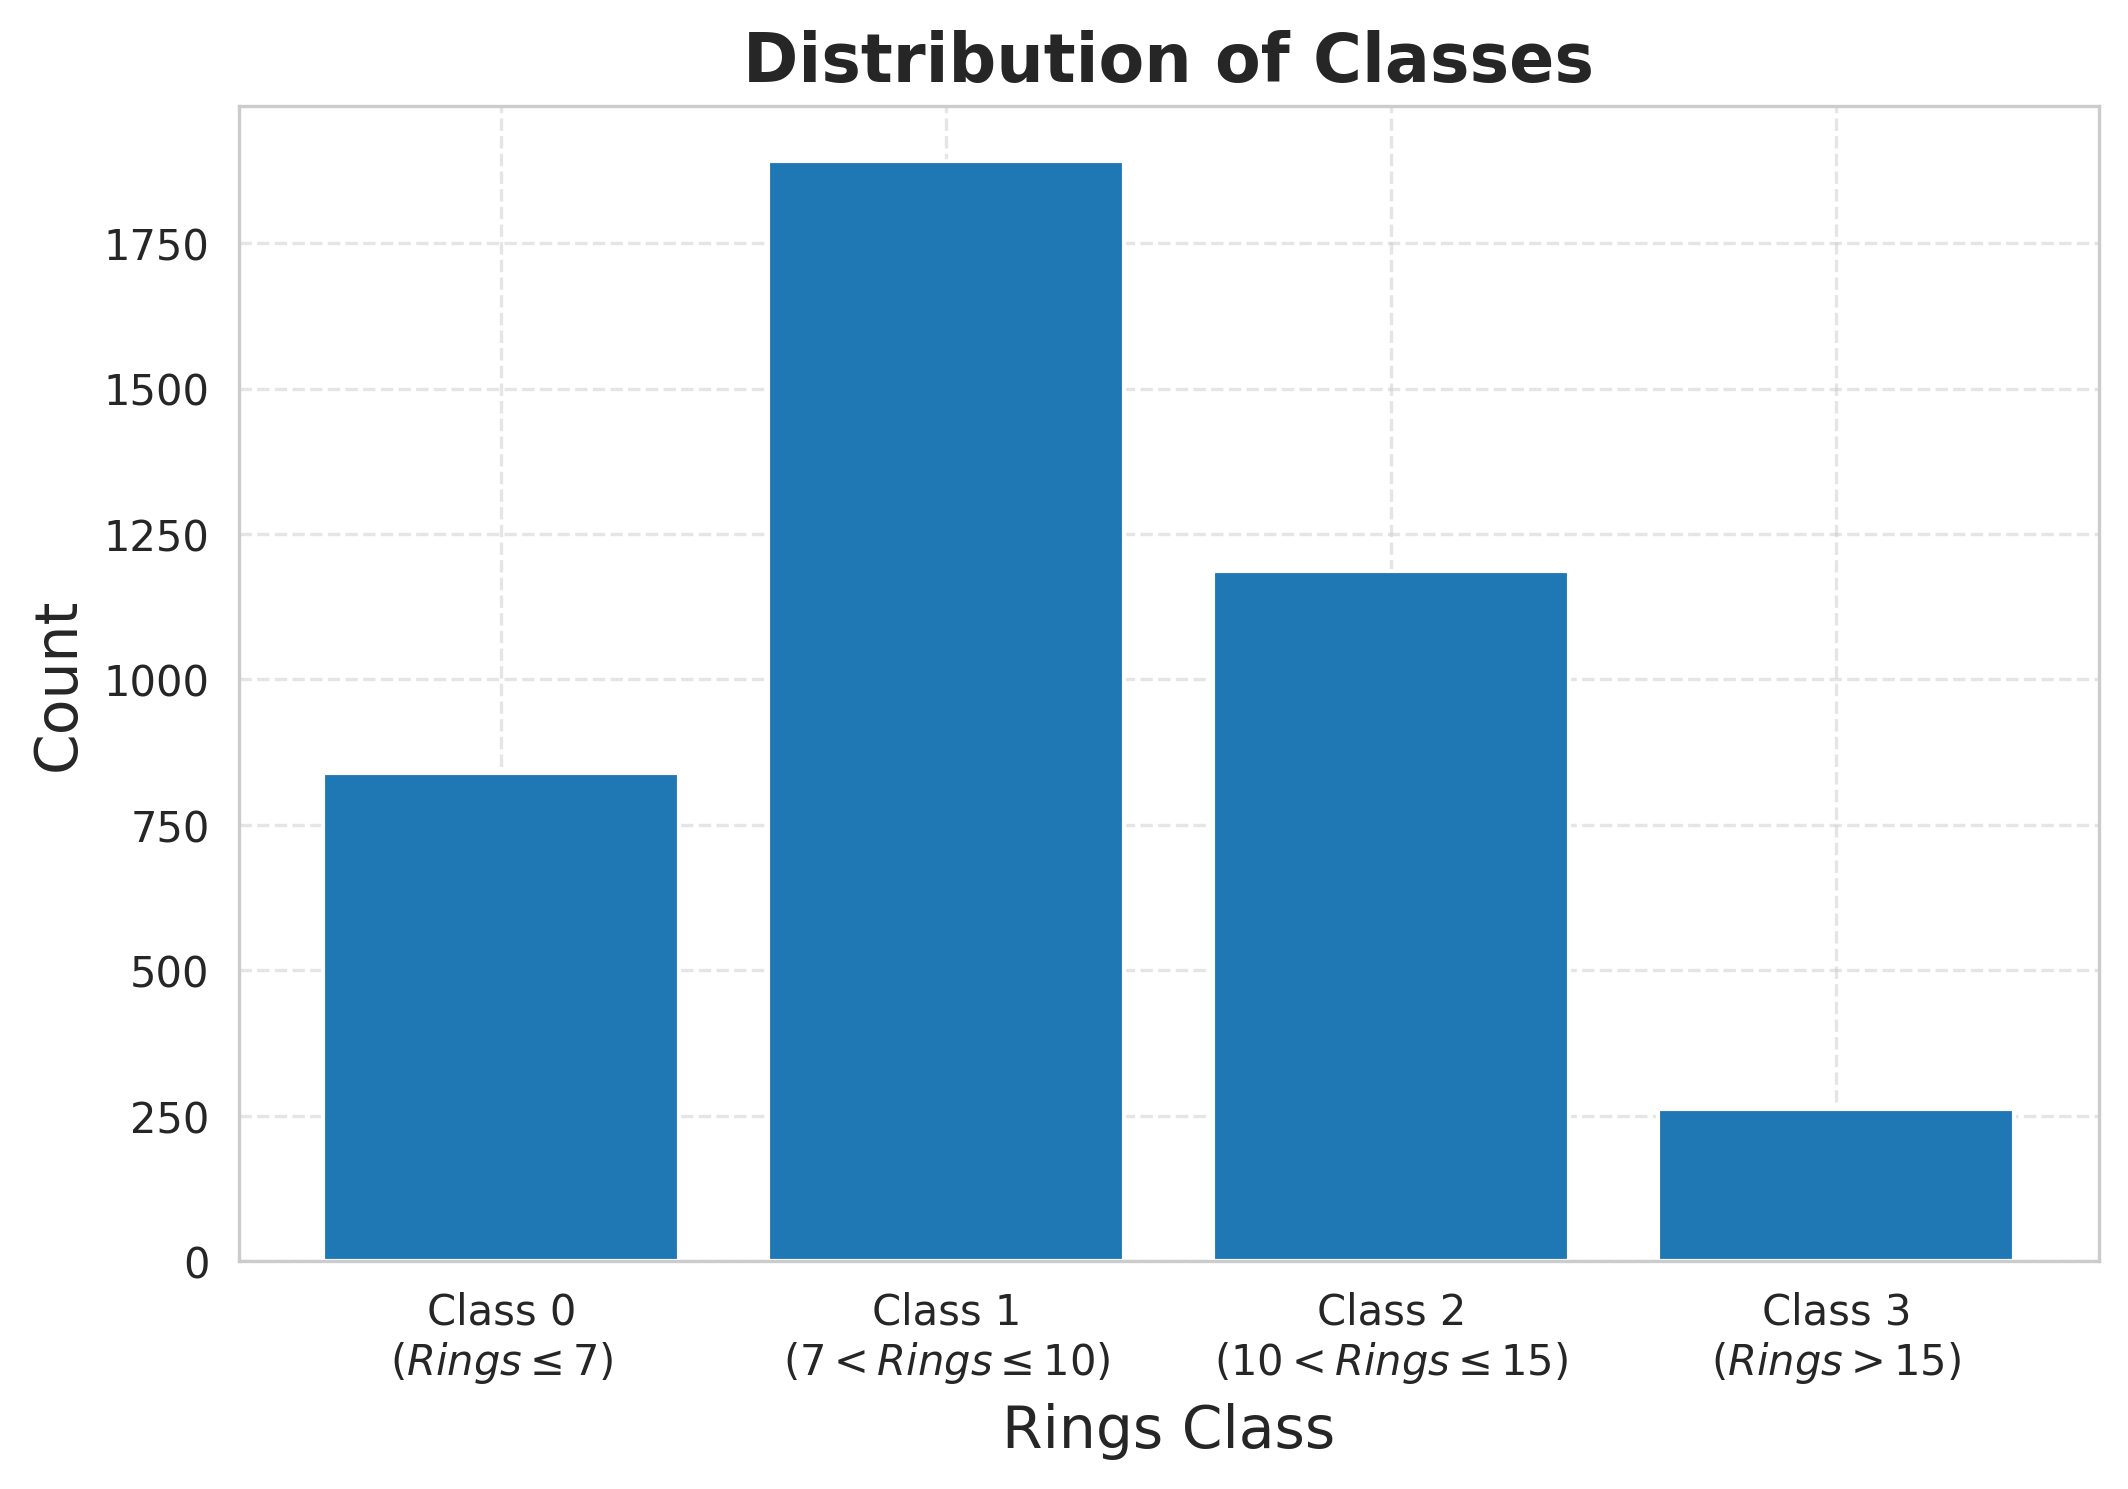
\includegraphics[width=0.8\linewidth]{ClassDistribution.png}
\caption{Distribution of classes of Rings}
\label{fig:classdist}
\end{figure}

There is an uneven distribution over the classes. Therefore, we ensured that any selection of train, test or validation data sets, used stratified sampling.


\begin{figure}[htbp]
\centering
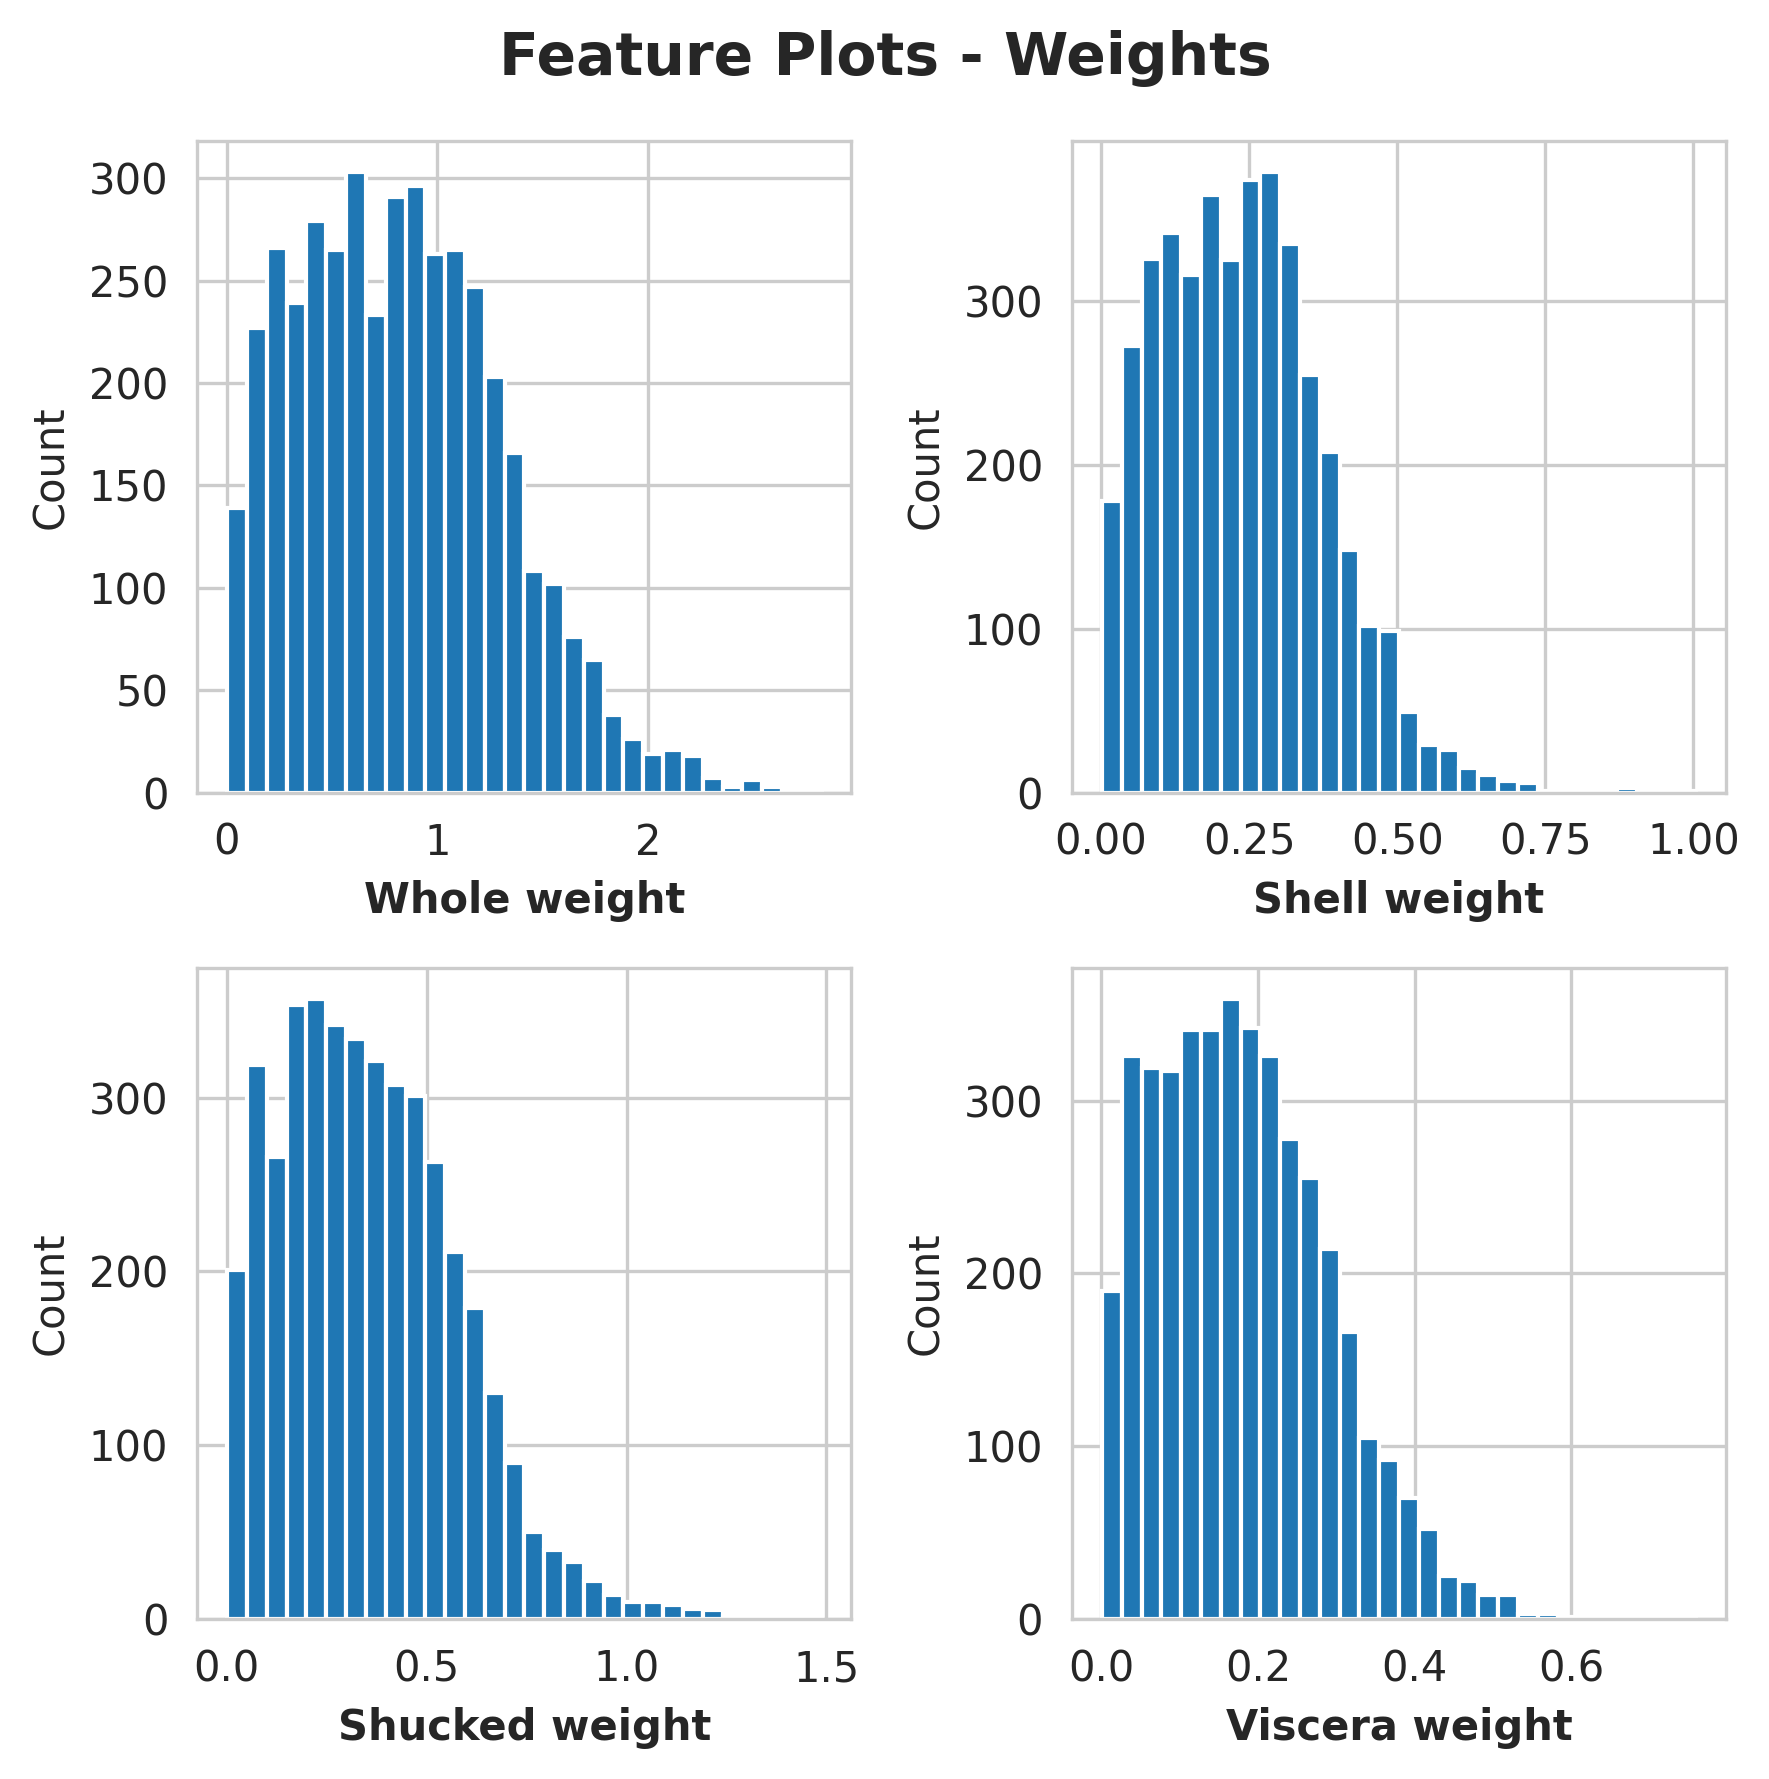
\includegraphics[width=1\linewidth]{Feature_plots_weights.png}
\caption{Distribution of Features: Weights}
\label{fig:feat_weight}
\end{figure}
Figure \ref{fig:feat_weight} shows that the distributions of weight related features are slightly right skewed, indicating weights are more concentrated towards the lower end. A smaller number of abalone with significantly larger weights pull the distribution towards the right. Although all continuous features in this dataset were divided by 200 for use with neural networks\textsuperscript{[1]}, these weight related features still have differing ranges, indicating a need for normalisation of the data prior to modelling. 

\begin{figure}[htbp]
\centering
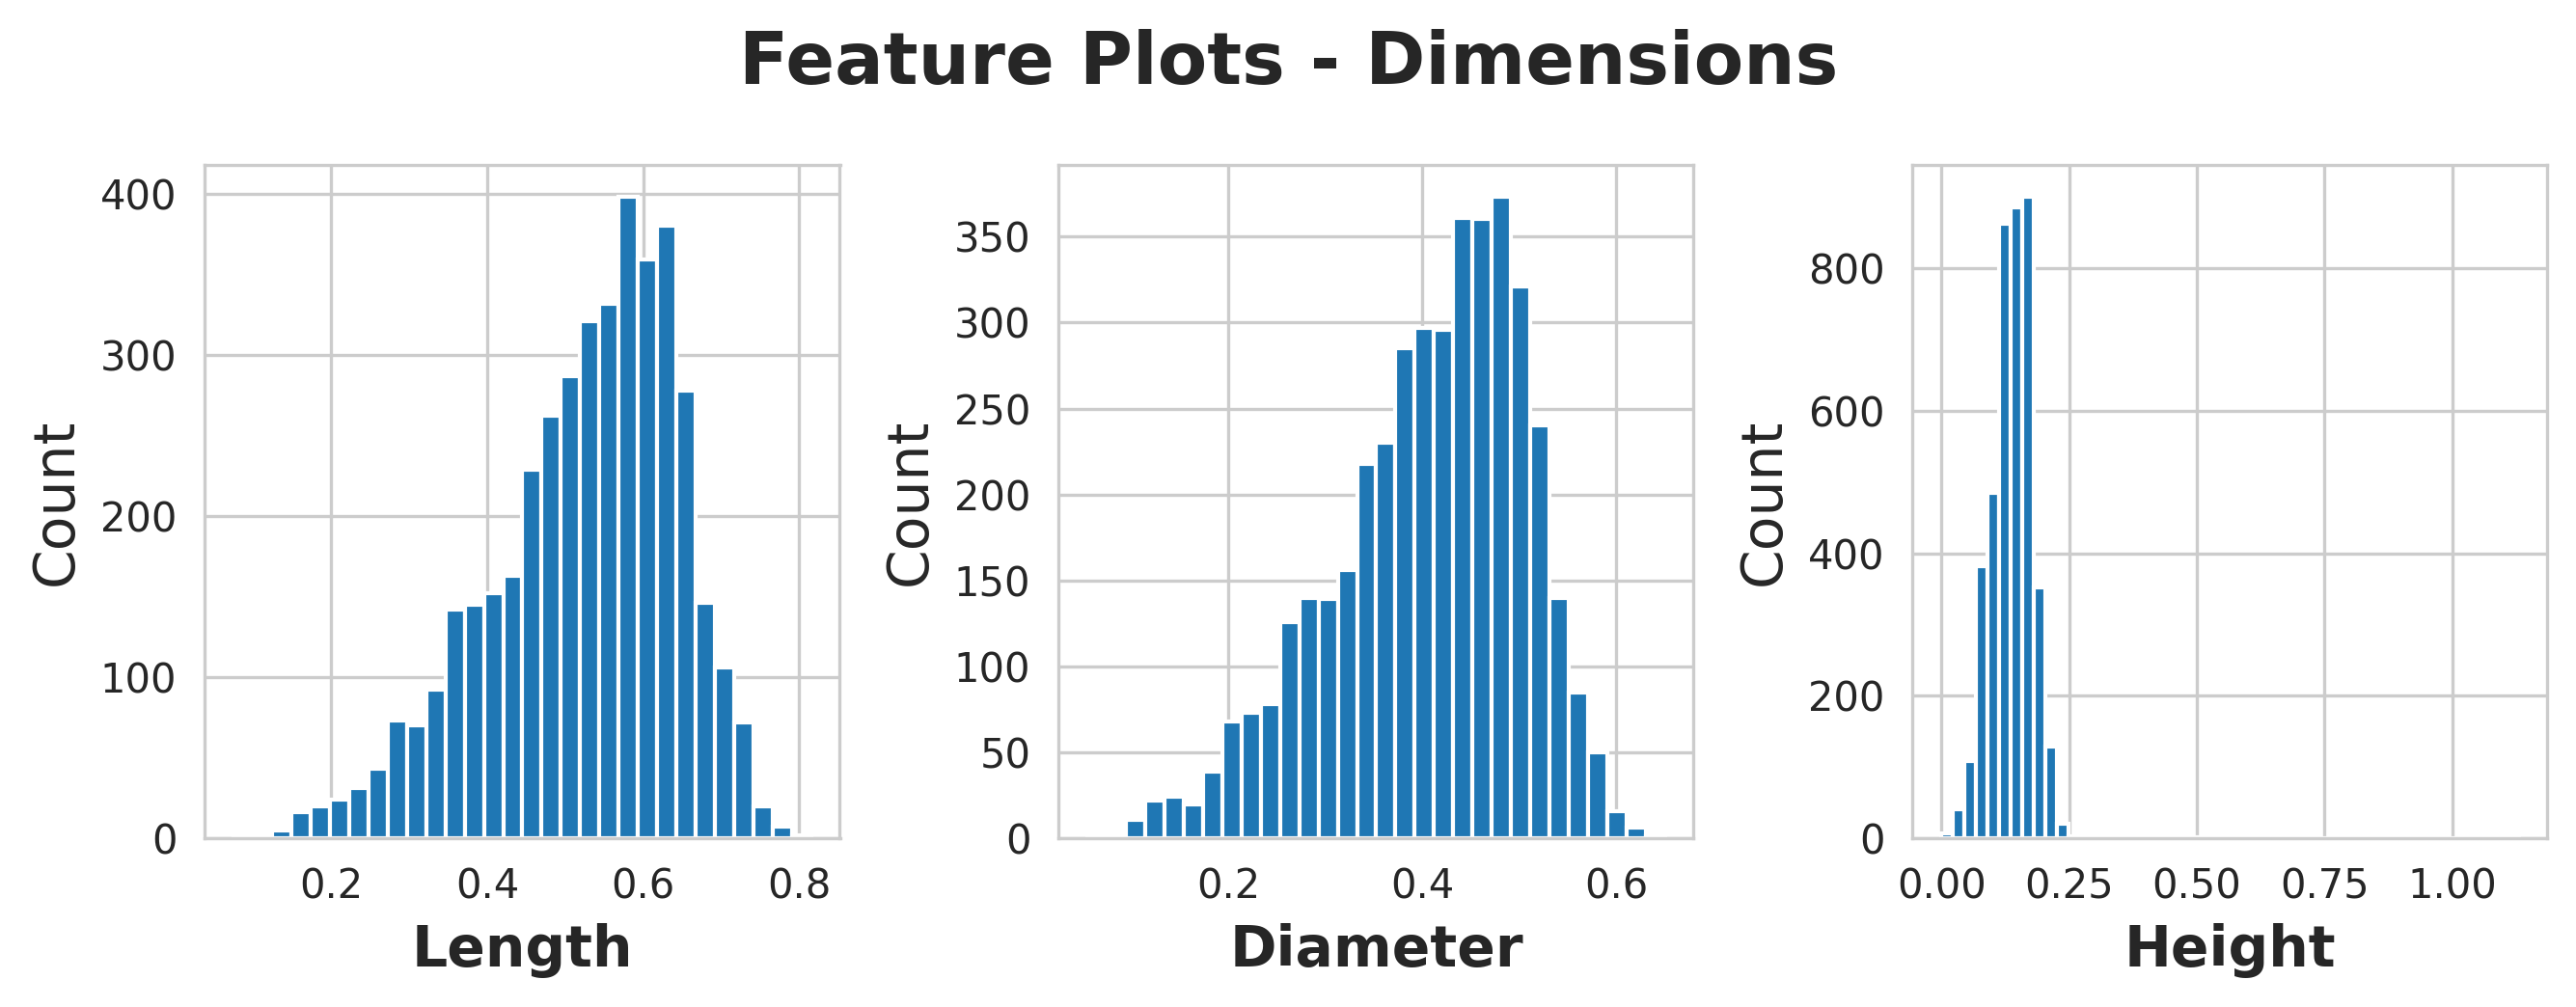
\includegraphics[width=1\linewidth]{Feature_plots_dimensions.png}
\caption{Distribution of Features: Dimensions}
\label{fig:feat_dim}
\end{figure}


Figure \ref{fig:feat_dim} shows that the distributions of dimension related features are slightly left skewed, indicating weights are more concentrated toward the higher end. \textit{Height} has 3 impossible outliers distorting the plot. 2 abalone have a height of 0 and 1 has height greater than length. The dataset defines length as the longest shell measurement\textsuperscript{[1]}, making it impossible for height to be greater than length. We removed these 3 impossible data points prior to modelling. The outliers can be seen in the \textit{Length vs. Height} plot in Figure \ref{fig:feat_out}. There are other outliers that can be seen in the plot, but these will be left in as biological anomalies rather than impossibilities.

\begin{figure}[htbp]
\centering
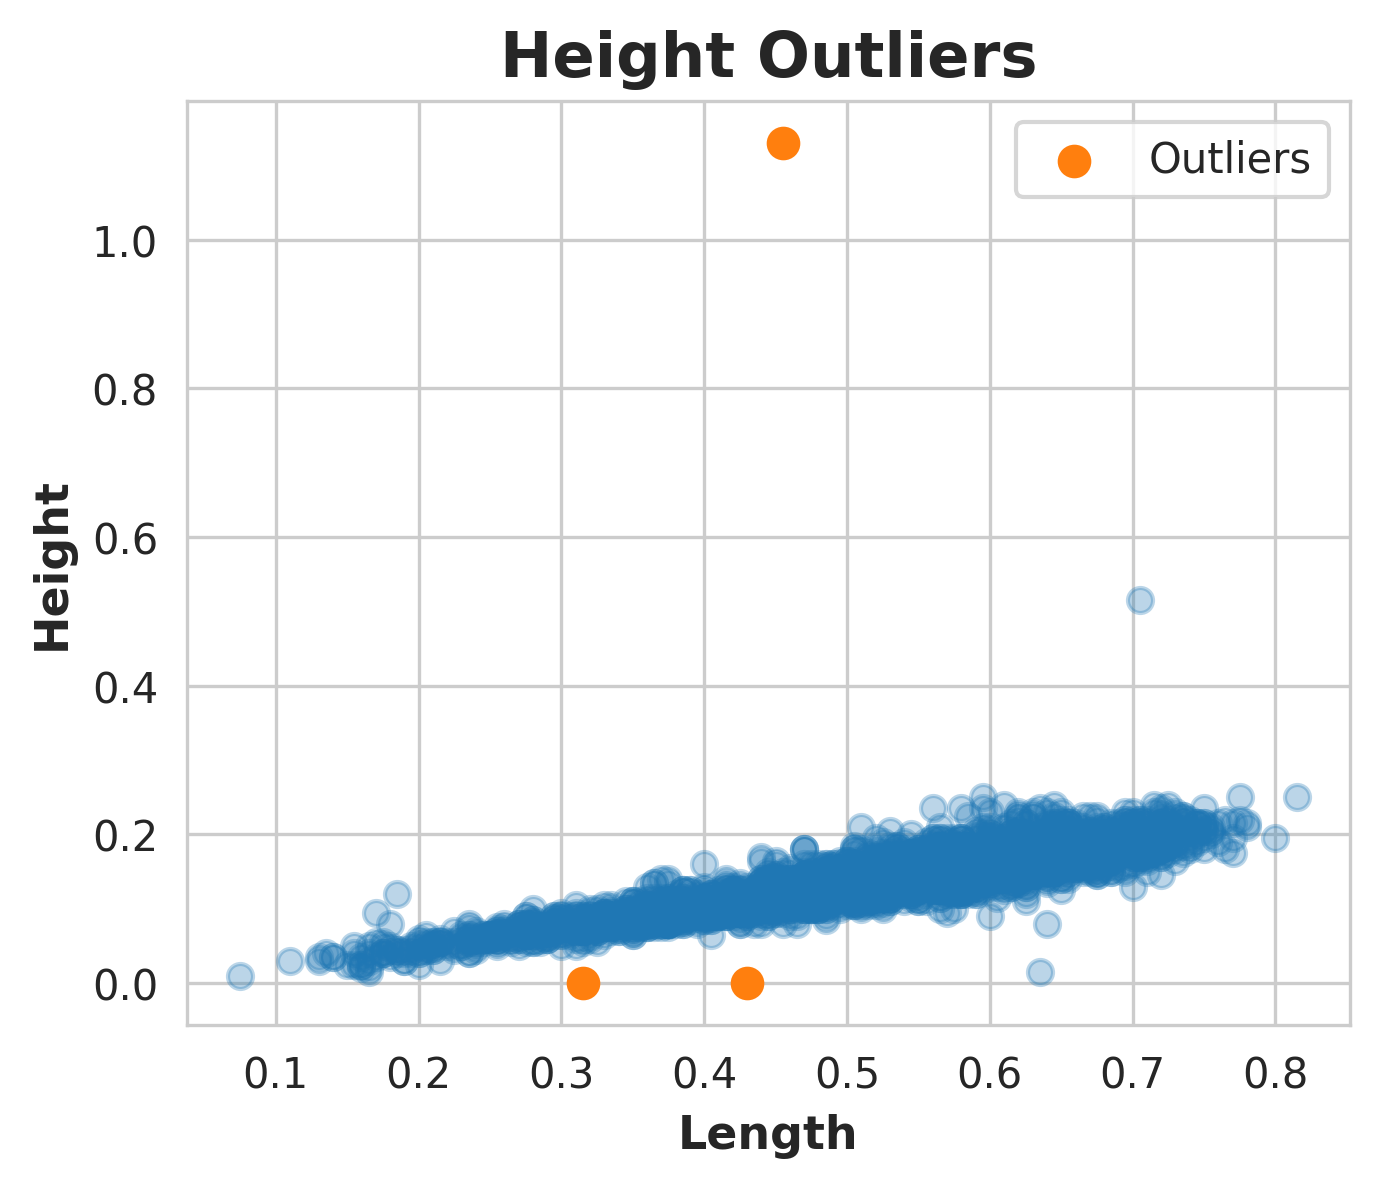
\includegraphics[width=0.8\linewidth]{Feature_plots_outliers.png}
\caption{Height Outliers}
\label{fig:feat_out}
\end{figure}

\text{}

The distribution of \textit{Sex} in Figure \ref{fig:feat_sex} shows a relatively even spread across the classes. The only required processing was one-hot coding these values as they were categorical string variables (I, M, F).

\begin{figure}[htbp]
\centering
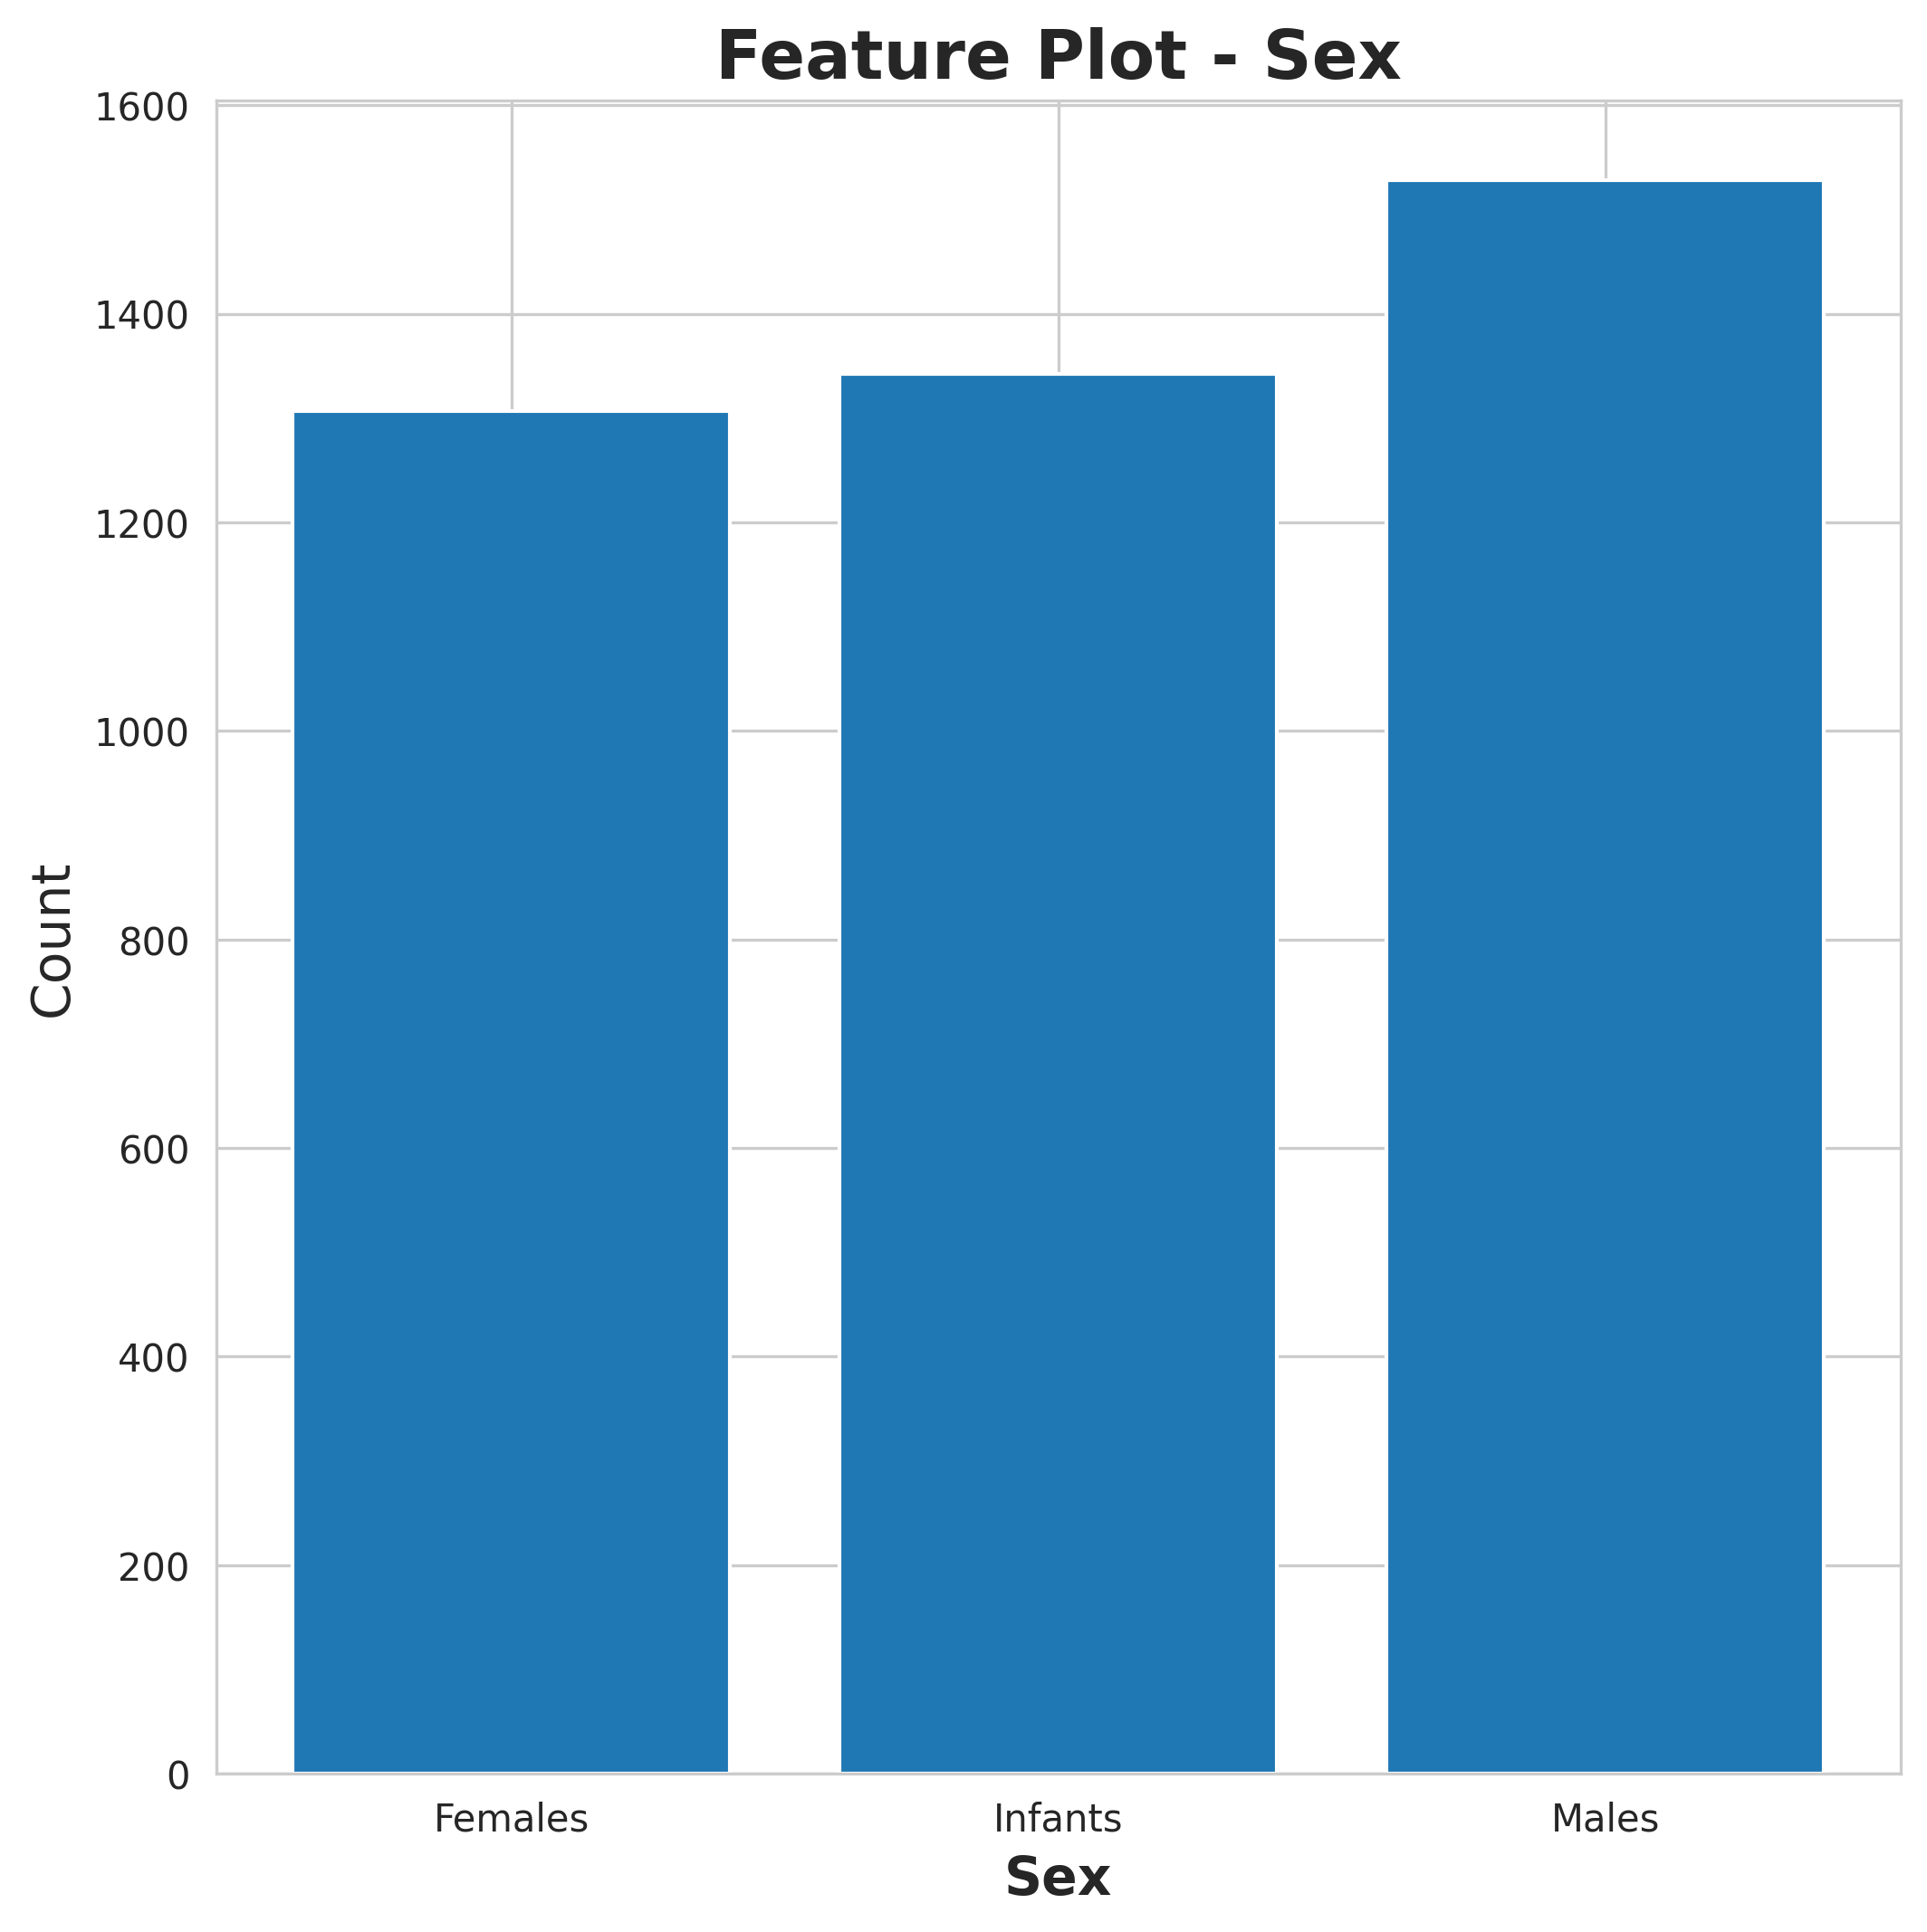
\includegraphics[width=0.7\linewidth]{Feature_plots_sex.png}
\caption{Distribution of Feature: Sex}
\label{fig:feat_sex}
\end{figure}

Continuous features were standardised with z-score standardisation to centre the data and promote better neural network training performance\textsuperscript{[3]}. \textit{Sex} was one-hot coded into three columns that could be used for training: \textit{Sex\_M} (males), \textit{Sex\_F} (females) and \textit{Sex\_I} (infants).

After standardisation, we split the full dataset into a training set and test set including 60\% and 40\% of data, respectively.


\text{}

\text{}

\text{}

\text{}
\subsection{Variable hyperparameter selection}
Hyperparameters were tuned sequentially, in the order below. We tuned 2 sets of these hyperparameters - 1 for each of the 2 optimisers we tested: SGD (Stochastic Gradient Descent) and Adam (Adaptive Moment estimation). Note, we used the mini-batch form of SGD but will refer to it as SGD throughout this report. 
\begin{enumerate}
    \item \textbf{Number of neurons per hidden layer}: Tested with 5, 10, 15 and 20 neurons. This explores range of neurons without vastly slowing training. 
    \item \textbf{Learning rate}: Tested with $10^x$ for \mbox{$x\in[-4, -1]$}, with a step size of $0.2$. This explores a range of learning rates from $10^{-4}$ to $10^{-1}$ on a logarithmic scale, allowing efficient testing of learning rates from multiple orders of magnitude.
    \item \textbf{Number of layers}: Tested with 1 and 2 layers. This explores the effect of adding 1 hidden layer on model performance.
\end{enumerate}
Each hyperparameter was tuned separately, and  the value which produced the best performing model was held fixed when tuning the next hyperparameter.
When tuning the number of neurons per hidden layer, we held the learning rate and the number of hidden layers fixed at 0.01 and 1, respectively. When tuning learning rate, we held the number of hidden layers fixed at 1. This allowed us to feasibly tune each hyperparameter sequentially, using valid default values, without testing every combination of these 3 hyperparameters.

We conducted 10 experiments for each hyperparameter value. Each experiment included re-training a model independently, 10 times, evaluating it with our test set and storing the train and test accuracies. This helped account for variance when selecting the best hyperparameter value.

We conducted paired t-tests to select the best hyperparameter values for the number of neurons per hidden layer and the number of hidden layers. In general, we prefer simpler models if performance is equal because it will help avoid overfitting\textsuperscript{[5, p. 463]}. Therefore, we selected the lowest value that produced mean test accuracies that were statistically equal to the best model. As we have no preference on the value of the learning rate once tuned, we selected the value which produced the model with the highest mean test accuracy.

\subsection{Fixed hyperparameter selection}
We held batch size and number of epochs fixed throughout all our experiments. This allowed us to focus on the effects of our variable hyperparameters.  

Batch size was fixed at 32 as it would provide good enough model performance for our tests and faster training times than smaller batch sizes\textsuperscript{[4]}.

Number of epochs was fixed at 103 after preliminary testing. 
We conducted this testing as follows: 
\begin{enumerate}
    \item Created temporary training and validation sets including 80\% and 20\% of full training set, respectively.
    \item Selected a naive mode to test. This model used 20 neurons per hidden layer, 2 hidden layers, a learning rate of $10^{-3}$ and the SGD optimiser.
    \item Trained 20 independent models to 400 epochs, storing train accuracy and validation accuracy metrics at each epoch.
    \item Averaged training and validation accuracy of all models at each epoch.
    \item Approximated growth rate as the difference between forward and backward moving averages, each with windows of 10 epochs.
    \item The epoch where growth fell below 0.5\% and the standard deviation of validation accuracy in the 20 epoch range was below 0.001 (0.1\% deviation), was set as the plateau point. This point was used as the constant number of epochs for all our tests.
\end{enumerate}
Our naive model was chosen as the slowest converging model we would be testing, except with a learning rate of $10^{-3}$ (the slowest model we actually tested had a learning rate of $10^{-4}$). This helped the naive model learn faster. This meant the plateau point would  occur at an epoch where the effect of overfitting on faster converging models, would not be evident.

A. Taşdelen has shown that patience criteria of 5, 7, 10 and 15 do not provide significantly different validation accuracy\textsuperscript{[7, p. 120]}. However, we wanted to ensure we captured a conservative range of epochs to model with. Our growth rate calculation and standard deviation requirement over the larger window of 20 epochs, allowed the plateau point to occur at a versatile epoch that could be used for all our upcoming experiments. This also helped prevented overfitting on simpler, faster converging models and underfitting on our more complex, slower converging models. Checking that standard deviation was below 0.001 ensured that accuracy varied very little over the range, asserting that any low growth was caused by true convergence rather than random fluctuations in accuracy.

\begin{figure}[htbp]
\centering
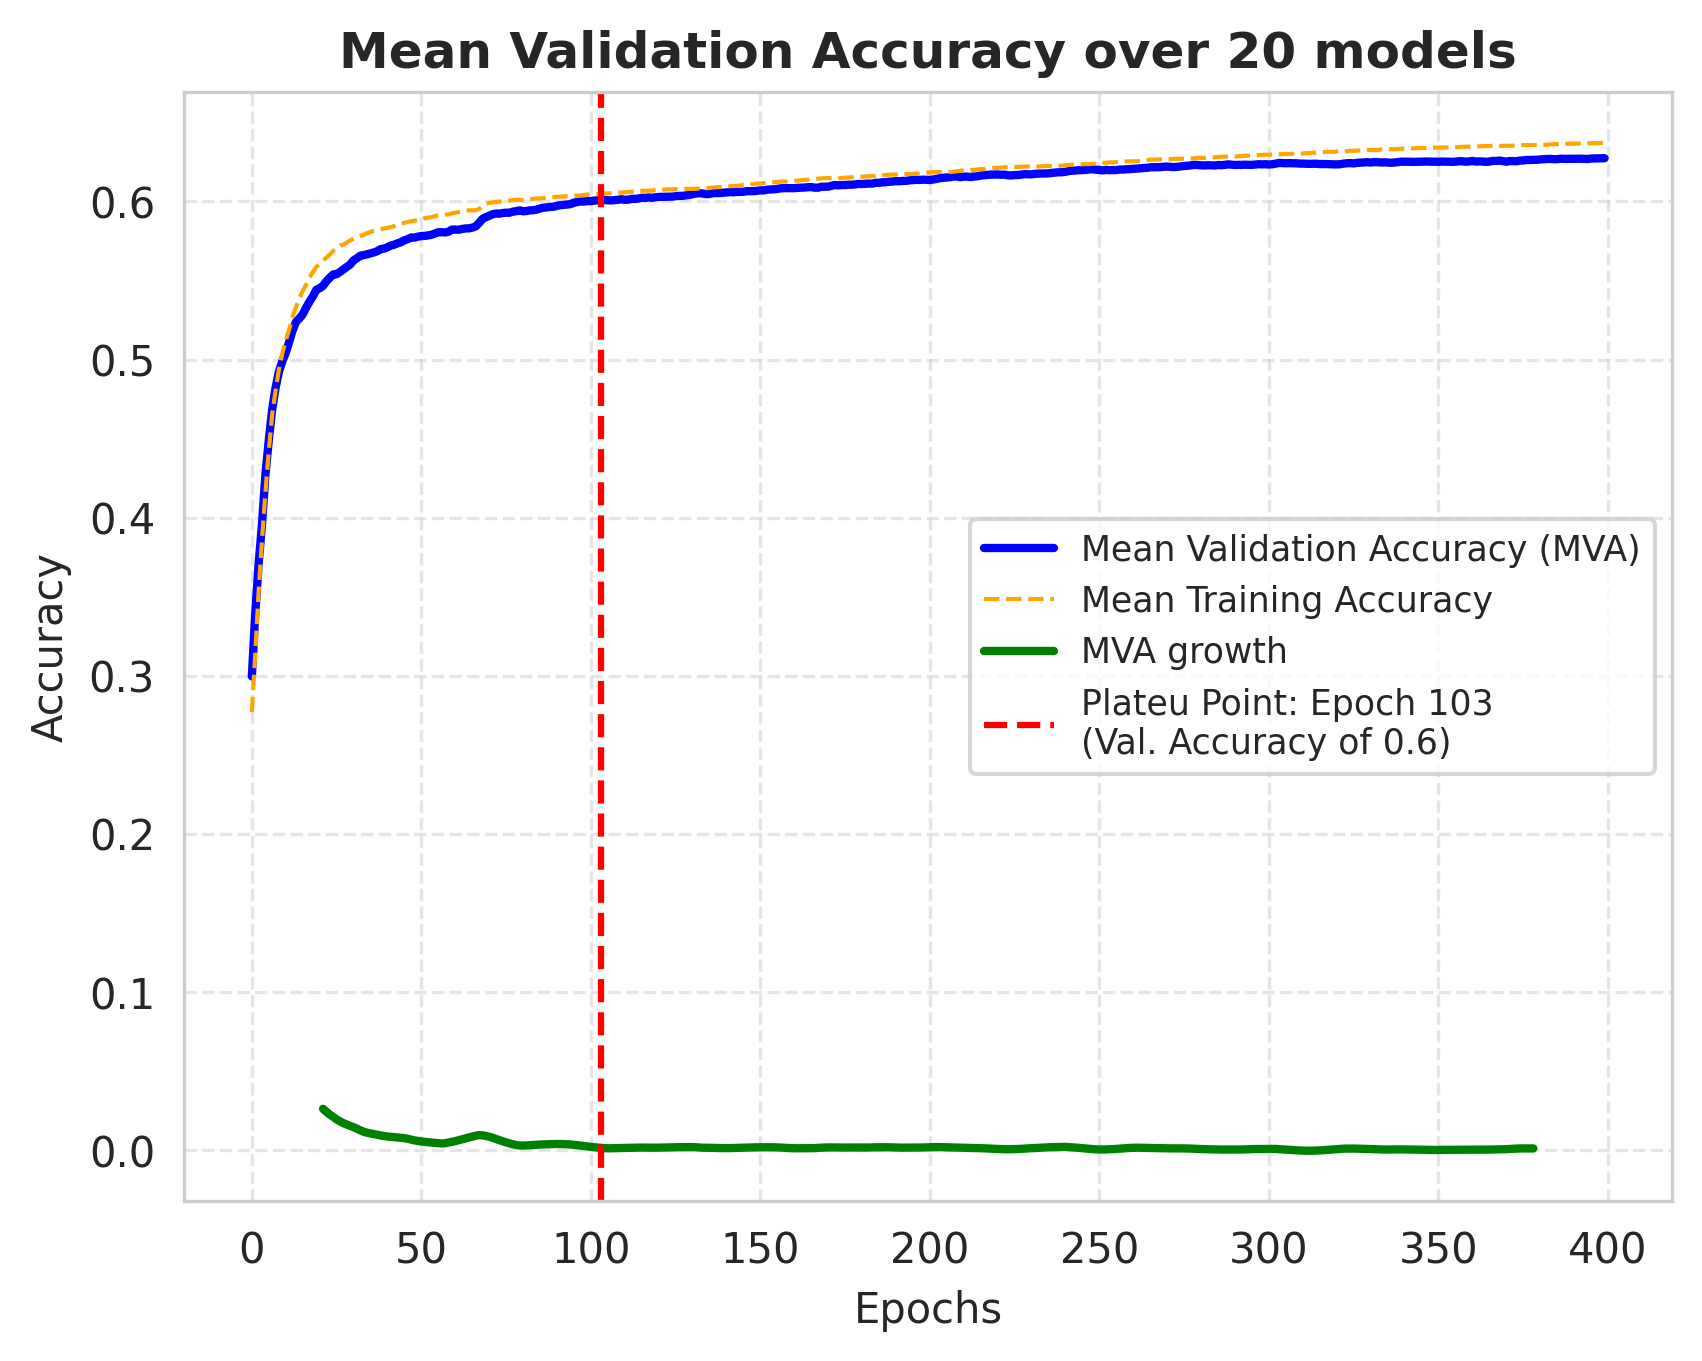
\includegraphics[width=1\linewidth]{Plateau.png}
\caption{Mean validation accuracy}
\label{fig:plateau}
\end{figure}

We can see in Figure \ref{fig:plateau} that mean train accuracy and mean validation accuracy stayed very similar over the training range indicating there is no blatant overfitting or underfitting, on average. However, both accuracies begin to diverge around epoch 300, indicating overfitting may become a problem if we used more than 400 epochs for training. 

Although accuracy continues to rise after the plateau point, the growth rate does not rise above 0.5\% again - in fact growth rate fell below 0.5\% at epoch 74 and never rose above 0.5\% again (standard deviation did not fall below 0.001 until epoch 103). The validation accuracy of this naive model at epoch 103 was 0.6. We selected hyperparameters based on models that were trained to this epoch.

\section{Results}
All tables report the top 10 models ranked in descending order of mean test accuracy.
\subsection{Optimiser: SGD (Stochastic Gradient Descent)}


\begin{table}[h]
\caption{SGD: Metrics for number of neurons per hidden layer}
\begin{center}
\renewcommand{\arraystretch}{1.3}
\begin{tabular}{|c|c|c|c|}
\hline
\textbf{Number of} & \multicolumn{2}{|c|}{\textbf{Mean Test results}}& \multirow{2}{*}{\textbf{p-value}} \\
\cline{2-3} 
\textbf{neurons} & \textbf{\textit{Accuracy}} & \textbf{\textit{95\% Confidence interval}} & \\
\cline{1-4}
\text{20}& \text{0.6194} &\text{(0.6161, 0.6227)} &\text{-} \\ 
\cline{1-4} 
\text{15}& \text{0.6187} &\text{(0.6158, 0.6217)} &\text{0.7772} \\ 
\cline{1-4} 
\text{10}& \text{0.6172} &\text{(0.6137, 0.6207)} &\text{0.3382} \\ 
\cline{1-4} 
\text{5}& \text{0.6084} &\text{(0.6016, 0.6151)} &\text{0.0109} \\ 
\hline 
\end{tabular}
\label{sgdhn}
\end{center}
\end{table}

Table \ref{sgdhn} shows the results of evaluation of different numbers of neurons per hidden layer. 

20 neurons in the hidden layer provides the best mean test accuracy. $p > 0.05$ for independent paired t-tests between the best model (20 neurons) and the 15 and 10 neuron models.  Therefore, we fail to reject the null that mean test accuracies of the 15 and 20 neuron models are equal. The same can be said for the 10 and 20 neuron models. We prefer simpler models, and the 10 neuron model provides mean test accuracies that are statistically equal to the best model So, we hold 10 neurons fixed as the most optimal number of neurons per hidden layer for SGD.


\begin{table}[h]
\caption{SGD: Metrics for learning rate}
\begin{center}
\renewcommand{\arraystretch}{1.3}
\begin{tabular}{|c|c|c|c|}
\hline
\multirow{2}{*}{\textbf{Learning Rate}} & \multicolumn{2}{|c|}{\textbf{Mean Test results}} &\multirow{2}{*}{\textbf{p-value}}\\
\cline{2-3} 
& \textbf{\textit{Accuracy}} & \textbf{\textit{95\% Confidence interval}} &\\
\hline
\text{$10^{-2.4}$}& \text{0.6369} &\text{(0.6336, 0.6403)} & -\\ 
\hline 
\text{$10^{-2.6}$}& \text{0.6367} &\text{(0.6339, 0.6395)} & 0.8982\\ 
\hline
\text{$10^{-2.8}$}& \text{0.6354} &\text{(0.6335, 0.6372)}& 0.2740\\ 
\hline
\text{$10^{-1.6}$}& \text{0.6348} &\text{(0.6309, 0.6386)}& 0.2674\\ 
\hline
\text{$10^{-1.8}$}& \text{0.6347} &\text{(0.6304, 0.6391)}& 0.4033\\ 
\hline 
\text{$10^{-3.0}$}& \text{0.6341} &\text{(0.6313, 0.6369)}& 0.2640\\ 
\hline
\text{$10^{-2.0}$}& \text{0.6328} &\text{(0.6294, 0.6362)}& 0.0926\\ 
\hline 
\text{$10^{-2.2}$}& \text{0.6323} &\text{(0.6282, 0.6365)}& 0.0694\\ 
\hline
\text{$10^{-1.4}$}& \text{0.6307} &\text{(0.6274, 0.6341)}& 0.0053\\ 
\hline
\text{$10^{-1.2}$}& \text{0.6292} &\text{(0.6219, 0.6365)}& 0.0508\\ 
\hline

\end{tabular}
\label{sgdlr}
\end{center}
\end{table}

Table \ref{sgdlr} shows the results of evaluation of different learning rates for our optimiser - SGD. A learning rate of $10^{-2.4}$ provides the best mean test accuracy and is fixed as the most optimal learning rate for our SGD tests.


\begin{table}[h]
\caption{SGD: Metrics for hidden layers}
\begin{center}
\renewcommand{\arraystretch}{1.3}
\begin{tabular}{|c|c|c|c|}
\hline
\textbf{Number of} & \multicolumn{2}{|c|}{\textbf{Mean Test results}}& \multirow{2}{*}{\textbf{p-value}} \\
\cline{2-3} 
\textbf{hidden layers} & \textbf{\textit{Accuracy}} & \textbf{\textit{95\% Confidence interval}} & \\
\cline{1-4}
\text{2}& \text{0.6040} &\text{(0.5988, 0.6091)} &\text{-} \\ 
\cline{1-4} 
\text{1}& \text{0.6020} &\text{(0.5963, 0.6078)} &\text{0.6165} \\ 
\hline 
\end{tabular}
\label{sgdhl}
\end{center}
\end{table}

Table \ref{sgdhl} shows the results of evaluation of using an additional hidden layer. 2 hidden layers provides the best mean test accuracy. Since $p > 0.05$ for the paired t-test between the best model (2 hidden layers) and 1 hidden layer models, we fail to reject the null that mean test accuracies are equal. Again, we prefer simpler models, and the 1 hidden layer model provides mean test accuracies that are statistically equal to the best model. So, we hold 1 hidden layer fixed as the most optimal number of hidden layers for SGD.

\text{}

Our final SGD model was trained with 10 neurons, a learning rate of $10^{-2.4}$ and 1 hidden layer.


\subsection{Optimiser: Adam (Adaptive Moment Estimation)}


\begin{table}[h]
\caption{Adam: Metrics for number of neurons per hidden layer}
\begin{center}
\renewcommand{\arraystretch}{1.3}
\begin{tabular}{|c|c|c|c|}
\hline
\textbf{Number of} & \multicolumn{2}{|c|}{\textbf{Mean Test results}}& \multirow{2}{*}{\textbf{p-value}} \\
\cline{2-3} 
\textbf{neurons} & \textbf{\textit{Accuracy}} & \textbf{\textit{95\% Confidence interval}} & \\
\cline{1-4}
\text{10}& \text{0.6337} &\text{(0.6316, 0.6358)} &\text{-} \\ 
\cline{1-4} 
\text{15}& \text{0.6322} &\text{(0.6265, 0.6379)} &\text{0.6133} \\ 
\cline{1-4} 
\text{20}& \text{0.6322} &\text{(0.6283, 0.636)} &\text{0.1831} \\ 
\cline{1-4} 
\text{5}& \text{0.6268} &\text{(0.6191, 0.6345)} &\text{0.1079} \\ 
\hline 
\end{tabular}
\label{adamhn}
\end{center}
\end{table}

Table \ref{adamhn} shows that 10 neurons per hidden layer provides the best mean test accuracy. $p > 0.05$ for the independent paired t-tests between the best model (10 neurons) and the 15 and 20 neuron models. Therefore, we fail to reject the null that mean test accuracies of the 10 and 15 neuron models are equal. The same can be said for the 10 and 20 neuron models. We prefer simpler models and the 10 neuron model is both the simplest and the best model of the 3, so we hold 10 neurons fixed as the most optimal number of neurons per hidden layer for Adam.


\begin{table}[h]
\caption{Adam: Metrics for learning rate}
\begin{center}
\renewcommand{\arraystretch}{1.3}
\begin{tabular}{|c|c|c|c|}
\hline
\multirow{2}{*}{\textbf{Learning Rate}} & \multicolumn{2}{|c|}{\textbf{Mean Test results}} &\multirow{2}{*}{\textbf{p-value}}\\
\cline{2-3} 
& \textbf{\textit{Accuracy}} & \textbf{\textit{95\% Confidence interval}} &\\
\hline
\text{$10^{-1.6}$}& \text{0.6351} &\text{(0.6317, 0.6386)} & -\\ 
\hline 
\text{$10^{-1.8}$}& \text{0.6307} &\text{(0.6245, 0.6368)} & 0.2579\\ 
\hline
\text{$10^{-2.6}$}& \text{0.6292} &\text{(0.6238, 0.6346)} & 0.0654\\ 
\hline
\text{$10^{-1.4}$}& \text{0.6277} &\text{(0.6217, 0.6337)}& 0.0699\\ 
\hline
\text{$10^{-2.8}$}& \text{0.6266} &\text{(0.6216, 0.6315)}& 0.0244\\ 
\hline
\text{$10^{-2.2}$}& \text{0.6264} &\text{(0.6197, 0.6331)}& 0.0455\\ 
\hline
\text{$10^{-2.4}$}& \text{0.6262} &\text{(0.6199, 0.6326)}& 0.0362\\ 
\hline
\text{$10^{-1.2}$}& \text{0.6256} &\text{(0.6186, 0.6327)}& 0.0226\\ 
\hline
\text{$10^{-2.0}$}& \text{0.6255} &\text{(0.6192, 0.6318)}& 0.0149\\ 
\hline
\text{$10^{-3.0}$}& \text{0.6213} &\text{(0.6174, 0.6251)}& 9.48\times10$^{-6}$\\ 
\hline
\end{tabular}
\label{adamlr}
\end{center}
\end{table}
Table \ref{adamlr} shows that a learning rate of $10^{-1.6}$ provides the best mean test accuracy and is held fixed as the most optimal learning rater for our Adam tests.




\begin{table}[h]
\caption{Adam: Metrics for number of hidden layers}
\begin{center}
\renewcommand{\arraystretch}{1.3}
\begin{tabular}{|c|c|c|c|}
\hline
\textbf{Number of} & \multicolumn{2}{|c|}{\textbf{Mean Test results}}& \multirow{2}{*}{\textbf{p-value}} \\
\cline{2-3} 
\textbf{hidden layers} & \textbf{\textit{Accuracy}} & \textbf{\textit{95\% Confidence interval}} & \\
\cline{1-4}
\text{2}& \text{0.6301} &\text{(0.6241, 0.6361)} &\text{-} \\ 
\cline{1-4} 
\text{1}& \text{0.6298} &\text{(0.6261, 0.6335)} &\text{0.8770} \\ 
\hline 
\end{tabular}
\label{adamhl}
\end{center}
\end{table}

Table \ref{adamhl} shows the results of evaluation of using an additional hidden layer. 2 hidden layers provides the best mean test accuracy. Since $p > 0.05$ for the paired t-test between the best model (2 hidden layers) and 1 hidden layer models, we fail to reject the null that mean test accuracies are equal. Therefore, as we prefer simpler models, and the 1 hidden layer model provides mean test accuracies that are statistically equal to the best model, we hold 1 hidden layer fixed as the most optimal number of hidden layers for SGD.

\text{}

Our final Adam model is trained with 10 neurons, a learning rate of $10^{-1.6}$ and 1 hidden layer.

\subsection{SGD and Adam model comparison}

\begin{table}[h]
\caption{Final SGD train \& test Results}
\begin{center}
\setlength{\tabcolsep}{3pt}
\renewcommand{\arraystretch}{1.3}
\begin{tabular}{|c|c|c|c|c|}
\hline
\multirow{2}{*}{\textbf{Optimiser}} &\multicolumn{2}{|c|}{\textbf{Mean Train results}} & \multicolumn{2}{|c|}{\textbf{Mean Test results}} \\
\cline{2-5}
& \textbf{\textit{Accuracy}} & \textbf{\textit{95\% CI}} & \textbf{\textit{Accuracy}} & \textbf{\textit{95\% CI}} \\
\hline
Adam & \text{0.6584}& \text{(0.6536, 0.6631)} & \text{0.6294} &\text{(0.6223, 0.6365)}\\ 
\hline
SGD & \text{0.6347}& \text{(0.628, 0.6413)} & \text{0.6009} &\text{(0.5948, 0.607)}\\ 
\hline
\end{tabular}
\label{sgd_final}
\end{center}
\end{table}
Table \ref{sgd_final} shows metrics for the final SGD and Adam models. The Adam model has higher mean test accuracy. The paired t-test on mean test accuracy between the Adam and SGD model produced a p-value of 6.63\times10$^{-5}$. $p < 0.05$, so we reject the null that mean test accuracies are equal. As the Adam model has the highest mean test accuracy, we chose this method of optimisation to create our final model.

\subsection{Final model metrics}

A new model was trained using the optimised Adam model hyperparameters and used to complete our final evaluation.



\begin{table}[h]
\caption{Confusion Matrix}
\begin{center}
\renewcommand{\arraystretch}{1.3}
\begin{tabular}{c|c|c|c|c|c|}
\multicolumn{1}{c}{} & \multicolumn{1}{c}{}& \multicolumn{4}{c}{\textbf{Actual}}\\
\cline{3-6}
\multicolumn{2}{c|}{} & \textit{Class 0} & \textit{Class 1} & \textit{Class 2} & \textit{Class 3} \\ 
\cline{2-6}
\multirow{5}{*}{\rotatebox{90}{\textbf{Predicted}}}  & \textit{Class 0} & 238 & 95 & 2 & 0 \\ 
\cline{2-6}
& \textit{Class 1} & 55 & 532 & 167 & 2 \\ 
\cline{2-6}
& \textit{Class 2} & 5 & 205 & 244 & 21 \\ 
\cline{2-6}
& \textit{Class 3} & 0 & 14 & 66 & 24 \\ 
\cline{2-6}
& \textit{\textbf{Precision}} & \textbf{0.7987} & \textbf{0.6288} & \textbf{0.5094} & \textbf{0.5106} \\ 
\cline{2-6}
\end{tabular}
\label{cm}
\end{center}
\end{table}

\begin{figure}[htbp]
\centering
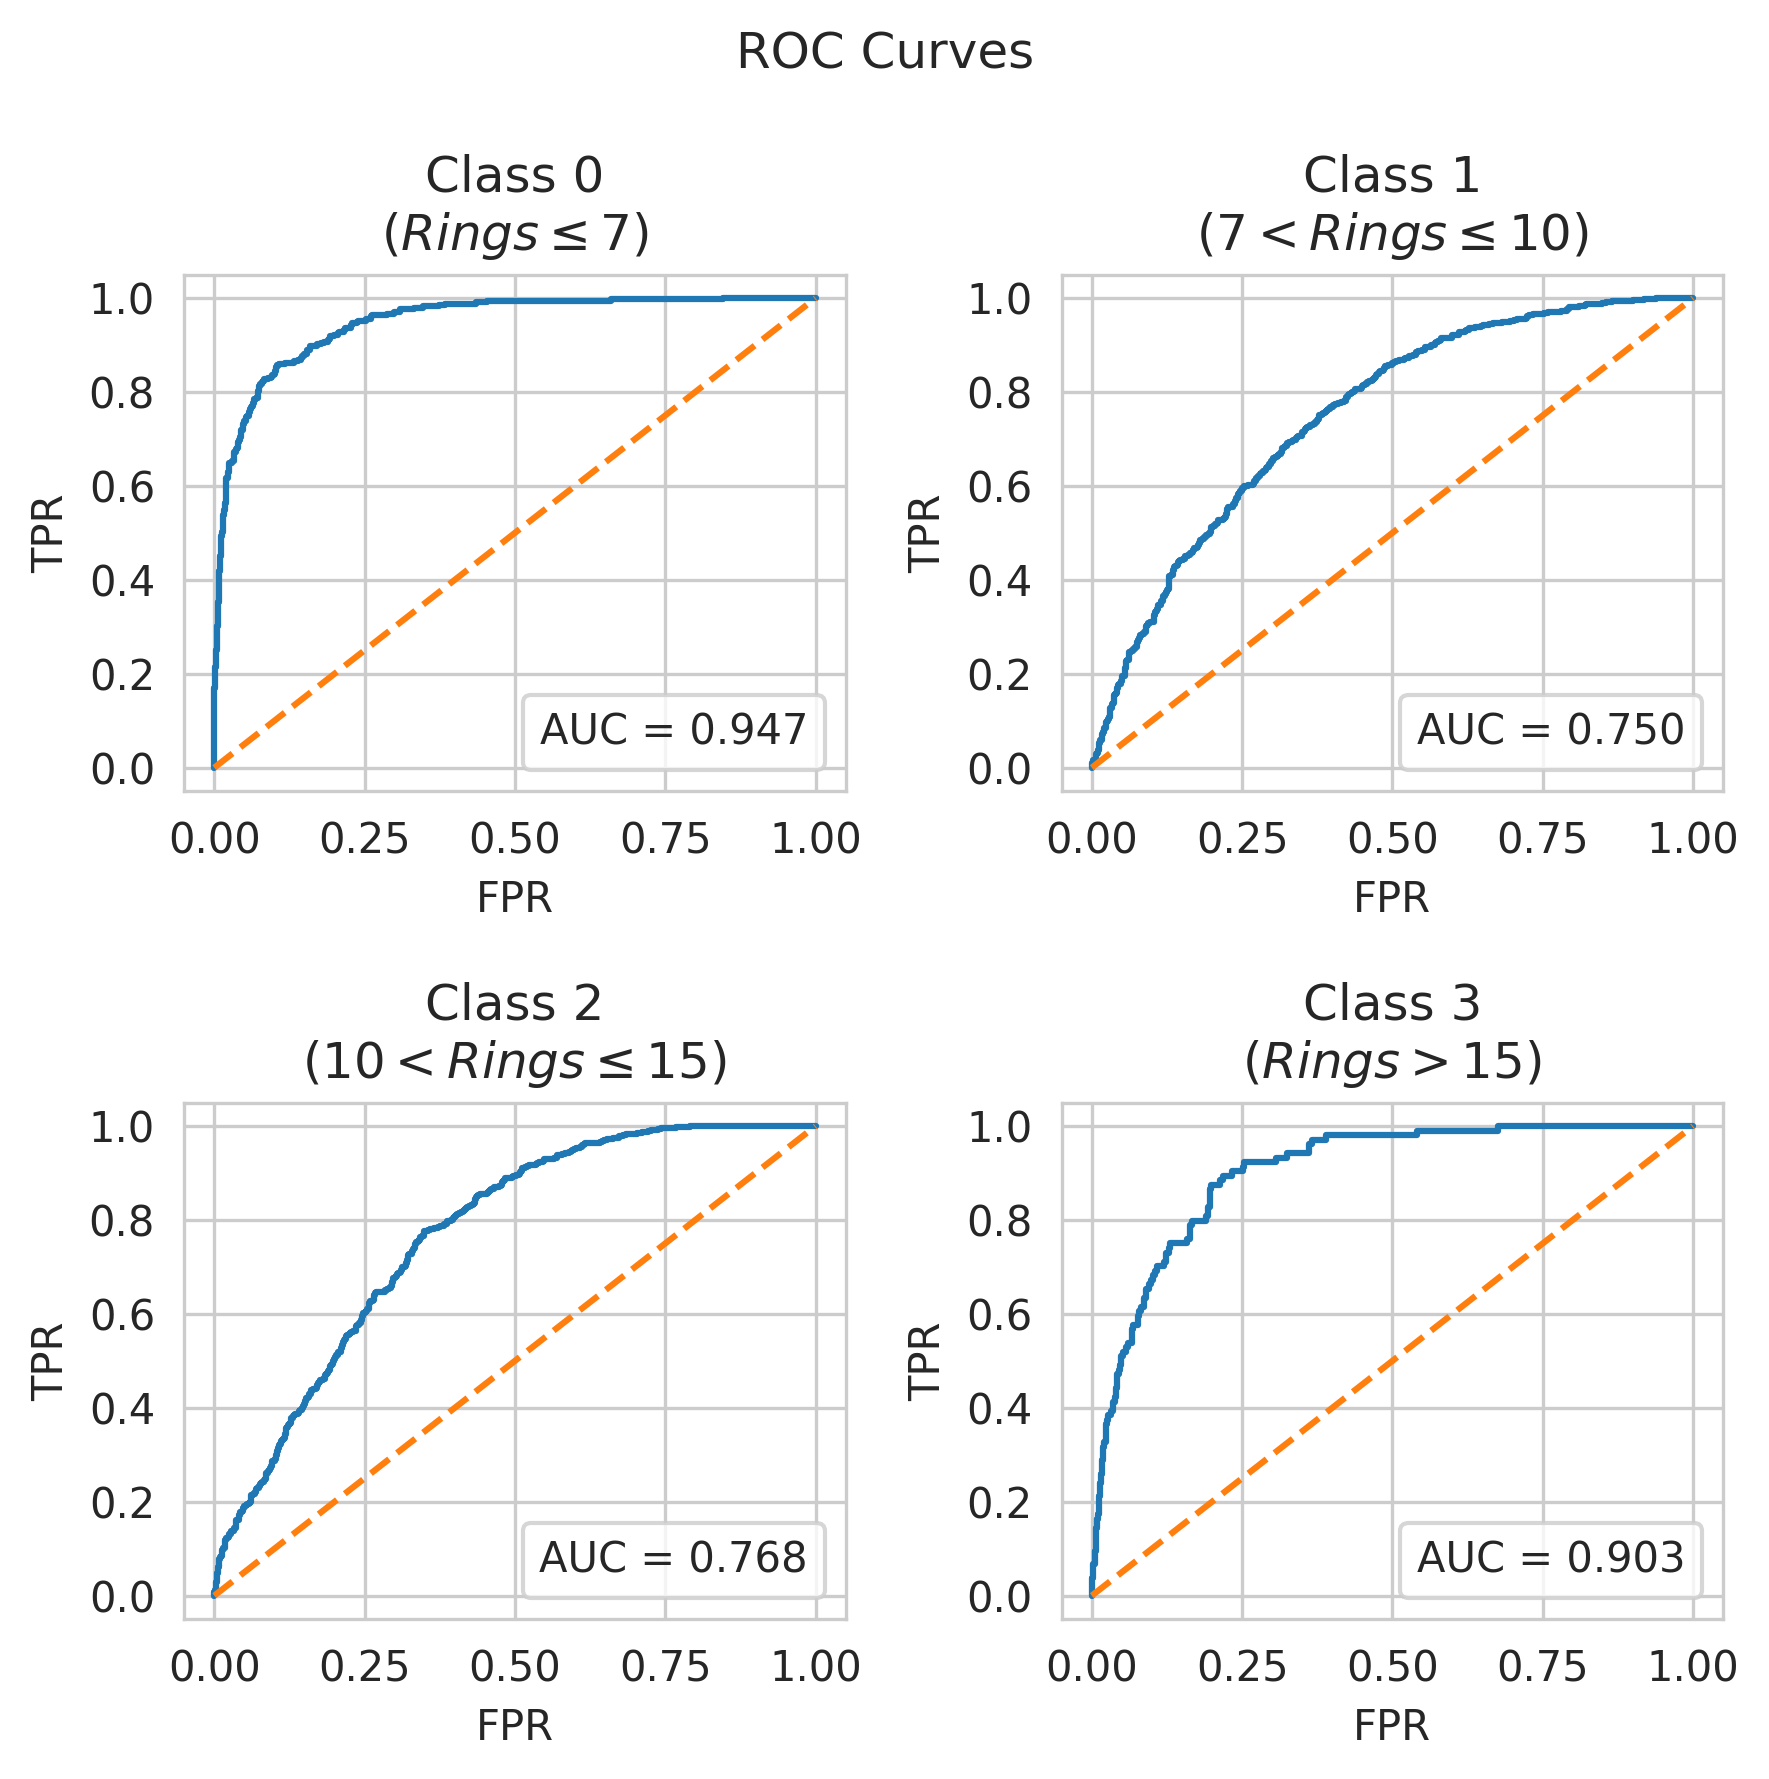
\includegraphics[width=1\linewidth]{ROC_curves.png}
\caption{ROC Curves}
\label{fig:roc}
\end{figure}
The confusion matrix and ROC curves for each of the classes are shown in Table \ref{cm} and Figure \ref{fig:roc}, respectively.

Precision of each class shows that predictions of Class 0 are reliable around 80\% of the time. Predictions of Class 1 are about 13\% more reliable than random guessing and predictions of Classes 2 and 3 are almost as reliable as random guessing. 

The ROC curves are promising, showing AUC to be 0.842 on average, across the 4 classes. 

\section{Discussion}
The results provide interesting insight into the need for hyperparameter tuning.

\text{}

\subsubsection{Neurons per hidden layer}


Our results in Tables \ref{sgdhn} and \ref{adamhn} showed that there is a plateau in model performance when increasing the number of neurons used. Tuning this parameter with both SGD and Adam showed that using 20 neurons over 15 neurons did not provide a statistically better mean test accuracy (at 5\% significance). SGD further showed that even compared to using 10 neurons, the 20 neuron model did not perform statistically better.

More neurons means more modelled features, but this also requires more computational power, time for training, and can lead to potential overfitting. These results assert the importance of optimising this parameter to create a well-performing model.

\text{}

\subsubsection{Number of hidden layers}
Through our results, we found that although using 2 hidden layers produced a better mean test accuracy, this result was not statistically different to using 1 hidden layer. Similar to the number of neurons per hidden layer, this hyperparameter plateaus early. Creating deeper models with more layers creates greater complexity leading to potential overfitting and greater training times. Again, this shows the importance of optimisaion of thes hyperparameters.

\text{}

\subsubsection{Learning Rate}
Tables \ref{sgdlr} and \ref{adamlr} showed that there is not necessarily a best learning rate. The 2nd to 6th best performing models for SGD and 2nd and 4th best learning rates for Adam all have $p > 0.05$ for their paired t-test with the model that used the best performing learning rate. So, we fail to reject the null that their mean test accuracies are equal to the best performing model. 
It seems our SGD model is not extremely sensitive to learning rate within a certain range - around 10$^-2$ to 10$^-3$. The Adam model however, seems adaptable to a wide range of learning rates. It seems optimising learning rate may not be as important as other hyperparameters on a simple feed-forward neural network like ours.

\text{}

\subsubsection{Optimiser}
In our discussion of Table \ref{sgd_final}, we noted that the model created using Adam had better performance. Since SGD tends to perform and converge better than alot of adaptive gradient algorithms like Adam in deep learning contexts\textsuperscript{[9, p. 1]}, it seems to be a perk of our model's simplicity that Adam performs better. We have seen that choosing this parameter carefully can greatly affect the final model performance with an almost 3\% difference in performance between our final SGD and Adam models.

\text{}

\subsubsection{Metrics}
The predictions of our model have poor precision on average and results should not be relied on to make decisions on the age of abalone. We can see that the model struggled the most when predicting Abalone belonging to Class 3 ($15 < \text{Rings}$) and Class 2 ($10 < \text{Rings} \leq 15$). 
The data contained the least amount of data points in Class 3 which may have caused poor generalisation towards that class. Class 2 may share many characteristics with Class 1 ($7 < \text{Rings} \leq 10$) and Class 3, causing confusion between the 2 classes. Class 1 had many more data points to train on than the other classes  hinting to why its recall is greater than Class 2. Class 0's high recall value indicates that there isn't much overlap with Class 1 to confuse the model. 

The AUC values for all our classes are relatively high. Class 0 and Class 3 especially have high AUCs at 0.947 and 0.903, respectively. This indicates the model can distinguish these classes from the others very well. Classes 1 and 2 have AUC of 0.750 and 0.768, respectively. Although the model is able to differentiate them from other classes, it is not at the level that is can differentiate Classes 0 and 3.


\section{Conclusion}
Undoubtedly, we have seen that correctly selecting hyperparameters is extremely important in maximising model performance. Some hyperparameters, like learning rate are less sensitive to changes within certain ranges. Others, like the number of neurons per hidden layer will plateau in performance relatively quickly, in basic models like our feed-forward neural network. Regardless, different values of these hyperparameters will optimise performance to create a better performing model and it is important these are optimised to fit the problem at hand.

There are many considerations left to explore. Data with a lot more classes and variables to map would benefit greatly from a much more complex model than we used and simple sequential tuning would exhaust much computational time. Even the traditional concept of the bias-variance tradeoff causing more complex models to overfit does not apply for the deep models being trained nowadays due to the concept of double descent\textsuperscript{[10, p. 2]}. In general, we must endeavour to treat neural networks as tools rather a self-sufficient problem solvers. In the same way the size of a screwdriver must be selected meticulously to remove or tighten a screw, we must meticulously select the hyperparameters used during training to build the right neural network for our problem.



\begin{thebibliography}{00}
\bibitem{b1} W. Nash, T. Sellers, S. Talbot, A. Cawthorn, and W. Ford,``Abalone," UCI Machine Learning Repository, 1994. Accessed: Apr. 10, 2026. doi: https://doi.org/10.24432/C55C7W.
\bibitem{b2} M. A. K. Raiaan et al., “A systematic review of hyperparameter optimization techniques in Convolutional Neural Networks,” Decision Analytics Journal, vol. 11, no. 100470, pp. 1-32, Apr. 2024. Accessed: Apr. 16, 2026. doi: https://doi.org/10.1016/j.dajour.2024.100470.
\bibitem{b3} M. Shanker, M.Y. Hu and M.S. Hung, ''Effect of data standardization on neural network training," Omega, vol. 24, no. 4, pp. 385-397, Feb. 1996. Accessed: Apr. 21, 2026. doi: https://doi.org/10.1016/0305-0483(96)00010-2.
\bibitem{b4} D. Masters and C. Luschi, “Revisiting Small Batch Training for Deep Neural Networks,” Apr. 2018. Accessed: Apr. 21, 2026. doi: https://arxiv.org/abs/1804.07612
\bibitem{b5} T. Deng, “Effect of the Number of Hidden Layer Neurons on the Accuracy of the Back Propagation Neural Network,” Highlights in science, engineering and technology, vol. 74, pp. 462–468, Dec. 2023. Accessed: Apr. 21, 2026. doi: https://doi.org/10.54097/nbra6h45.
\bibitem{b6} Yan Pan and Yuanzhi Li, “Toward Understanding Why Adam Converges Faster Than SGD for Transformers,” May. 2023. Accessed: Apr. 21, 2026. doi: https://doi.org/10.48550/arXiv.2306.00204
\bibitem{b7} A. Taşdelen, “Enhancing green computing through energy-aware training: an early stopping perspective,” Current trends in computing, vol. 2, no. 2, pp. 109-139 Dec. 2024. Accessed: Apr. 21, 2026 doi: https://doi.org/10.71074/ctc.1594291.
\bibitem{b8} D. Faraggi and R. Simon, “A neural network model for survival data,” Statistics in Medicine, vol. 14, no. 1, pp. 73–82, Jan. 1995. Accessed: Apr. 22, 2026 doi: https://doi.org/10.1002/sim.4780140108.
\bibitem{b9} P. Zhou, J. Feng, C. Ma, C. Xiong, Steven, and E Weinan, “Towards Theoretically Understanding Why SGD Generalizes Better Than ADAM in Deep Learning,” Oct. 2020. Accessed: Apr. 22, 2026. doi: 
https://doi.org/10.48550/arXiv.2010.05627.
‌\bibitem{b10} P. Nakkiran, G. Kaplun, Y. Bansal, T. Yang, B. Barak, and I. Sutskever, “Deep double descent: where bigger models and more data hurt,” Journal of Statistical Mechanics: Theory and Experiment, vol. 2021, no. 12, p. 124003, Dec. 2021. Access Apr. 23, 2026. doi: https://doi.org/10.1088/1742-5468/ac3a74.
\end{thebibliography}


\end{document}
